%*************************************
% บทที่ 4
%*************************************
\chapterTitle{4}{ผลการดำเนินงาน}

\hspace*{1.5em}
ในการพัฒนา Template สำหรับการจัดทำเล่มปริญญานิพนธ์ด้วย LaTeX จัดทำขึ้นเพื่ออำนวยความสะดวกให้แก่นักศึกษาในภาควิชาเทคโนโลยีสารสนเทศ ให้สามารถจัดรูปเล่มได้ถูกต้องตามรูปแบบมาตรฐานที่กำหนด ในส่วนของผลการดำเนินงานที่ได้ประกอบด้วยไฟล์โครงสร้างและการปรับแต่งรูปแบบเอกสาร
ตั้งแต่หน้าปก ปกในภาษาไทย ปกในภาษาอังกฤษ ใบรับรองปริญญานิพนธ์ บทคัดย่อภาษาไทย บทคัดย่อภาษาอังกฤษ กิตติกรรมประกาศ สารบัญ สารบัญภาพ สารบัญตาราง บทเนื้อหา บรรณานุกรม และภาคผนวก
ทั้งนี้ ผู้จัดทำได้ทดสอบการใช้งาน Template ดังกล่าว โดยตรวจสอบการจัดหน้า การอ้างอิง และรูปแบบการนำเสนอ เพื่อให้มั่นใจว่าสามารถนำไปใช้งานได้จริง สอดคล้องตามคู่มือการจัดทำเล่มวิทยานิพนธ์ของภาควิชา
\section{โครงสร้างโฟลเดอร์}
\hspace*{1.5em}
จากการออกแบบและพัฒนา Template ของรูปเล่มปริญญานิพนธ์ด้วย LaTeX ประกอบไปด้วย 3 โฟลเดอร์หลัก ได้แก่ 

\subsection{โฟลเดอร์ Class}
\hspace*{1.5em}
โฟลเดอร์ \textbf{Class} เป็นที่เก็บไฟล์รูปแบบเอกสารหลัก \textbf{project\_report.cls} เป็นไฟล์คลาส (Class File) ที่เขียนด้วยภาษา LaTeX มีหน้าที่กำหนดรูปแบบของการจัดรูปเล่มปริญญานิพนธ์ เช่น ขนาดกระดาษ และระยะขอบหน้า-หลัง รูปแบบและขนาดตัวอักษร รูปแบบบทและหัวข้อย่อย รวมทั้งการจัดวางสารบัญ ตาราง รูปภาพ และบรรณานุกรม

\subsection{โฟลเดอร์ Font}
\hspace*{1.5em}
โฟลเดอร์ \textbf{Font} ใช้สำหรับเก็บไฟล์ฟอนต์ที่จำเป็นต้องใช้ในการจัดรูปแบบรูปเล่มปริญญานิพนธ์ ภายในโฟลเดอร์นี้จะเก็บไฟล์ฟอนต์ \textbf{TH Sarabun New} ซึ่งเป็นฟอนต์ภาษาไทยมาตรฐาน 
ที่มีรูปแบบตัวอักษรชัดเจนและเหมาะสมสำหรับงานวิชาการ ตัวอย่างไฟล์ฟอนต์ที่เก็บ ได้แก่
\begin{mycustomenum2}
  \item \textbf{THSarabunNew.ttf}
  \item \textbf{THSarabunNew Bold.ttf}
  \item \textbf{THSarabunNew Italic.ttf}
  \item \textbf{THSarabunNew BoldItalic.ttf}
\end{mycustomenum2}
\hspace*{1.5em}
การเก็บฟอนต์ในโฟลเดอร์ \textbf{Font} จะช่วยให้โครงสร้างโปรเจกต์เป็นระเบียบ 
และสะดวกต่อการจัดการไฟล์ฟอนต์เมื่อย้ายไปใช้งานในเครื่องคอมพิวเตอร์อื่น ๆ 

\subsection{โฟลเดอร์ Image}
\hspace*{1.5em}
โฟลเดอร์ \textbf{Image} ใช้สำหรับเก็บไฟล์รูปภาพประกอบที่ใช้ในรูปเล่มปริญญานิพนธ์ โดยการแยกรูปภาพไว้ในโฟลเดอร์นี้จะช่วยให้การจัดการไฟล์ง่ายขึ้นและป้องกันความสับสนกับไฟล์อื่น ๆ เช่น ไฟล์โค้ดหรือไฟล์เอกสารหลัก โดยทั่วไปแล้วไฟล์รูปภาพที่ใช้ใน LaTeX ควรอยู่ในรูปแบบที่เหมาะสม เช่น PNG หรือ JPG เพื่อให้สามารถแสดงผลได้ถูกต้องและมีคุณภาพสูง

\section{โครงสร้างไฟล์}
\subsection{ไฟล์เอกสารหลัก}
\hspace*{1.5em}
นอกจากโฟลเดอร์ทั้งสามที่กล่าวมาแล้ว ในโครงสร้างโปรเจกต์ยังมีไฟล์เอกสารหลักที่สำคัญอีกหนึ่งไฟล์ คือ \textbf{Main.tex} ซึ่งเป็นไฟล์หลักที่ใช้ในการรวบรวมเนื้อหาทั้งหมดของปริญญานิพนธ์เข้าไว้ด้วยกัน ไฟล์นี้จะทำหน้าที่เรียกใช้ไฟล์คลาส (\textbf{project\_report.cls}) เพื่อกำหนดรูปแบบหน้ากระดาษ รวมถึงเรียกใช้เนื้อหาในแต่ละบท (เช่น บทนำ ทฤษฎีที่เกี่ยวข้อง วิธีการดำเนินงาน ผลการทดลอง) และองค์ประกอบอื่น ๆ เช่น สารบัญ สารบัญตาราง สารบัญรูปภาพ และบรรณานุกรม ทำให้ผู้ใช้งานสามารถจัดการเนื้อหาแต่ละส่วนได้อย่างเป็นระบบและง่ายต่อการแก้ไข

\subsection{ตัวอย่างโครงสร้างไฟล์ทั้งหมด}
\hspace*{1.5em}
ภาพที่ \ref{fig4:StructureFile} แสดงตัวอย่างโครงสร้างไฟล์ทั้งหมดที่ใช้ในการจัดทำรูปเล่มปริญญานิพนธ์ด้วย LaTeX จะเห็นว่ามีการจัดระเบียบไฟล์อย่างเป็นระบบ เพื่อความสะดวกในการจัดการและแก้ไขเนื้อหา โดยโครงสร้างประกอบด้วยโฟลเดอร์หลัก 3 โฟลเดอร์ ได้แก่ Class, Font และ Image ซึ่งทำหน้าที่เก็บไฟล์ที่เกี่ยวข้องกับการตั้งค่า รูปแบบตัวอักษร และรูปภาพตามลำดับ อีกทั้งยังมีไฟล์หลัก \textbf{Main.tex} และไฟล์คลาส (\textbf{project\_report.cls}) ดังที่กล่าวไว้ข้างต้น

\hspace*{1.5em}
นอกจากนี้ยังประกอบด้วยไฟล์หลักอีกหลายไฟล์ ได้แก่
\begin{mycustomitem}
    \item Project\_000\_Cover.tex สำหรับปก
    \item Project\_001\_Certificate.tex สำหรับใบรับรองปริญญานิพนธ์ ซึ่งจะมีด้วยกัน 2 ไฟล์ให้เลือกใช้ 
    \begin{mycustomitem}
        \item Project\_001\_Certificate1.tex ในกรณีไม่มีที่ปรึกษาร่วม และ 
        \item Project\_001\_Certificate2.tex กรณีมีที่ปรึกษาร่วม 
    \end{mycustomitem}
    (กำหนดที่ไฟล์ Main.tex)
    \item Project\_002\_Abstract.tex สำหรับบทคัดย่อ
    \item Project\_010\_Chapter1.tex สำหรับบทที่ 1 และ 
    \item Project\_999\_Bibliography.bib สำหรับบรรณานุกรม
\end{mycustomitem}
\hspace*{1.5em}
การแบ่งไฟล์เป็นส่วนย่อยเช่นนี้ช่วยให้การจัดการเนื้อหาแต่ละส่วนมีความเป็นระเบียบ และง่ายต่อการทำงานร่วมกันเป็นทีม เมื่อต้องการแก้ไขเนื้อหาในบทใดบทหนึ่งก็สามารถเข้าไปแก้ไขได้โดยตรงในไฟล์นั้น ๆ โดยไม่กระทบกับส่วนอื่น ๆ ของรูปเล่ม 

\begin{figure}[htbp]
\centering
\adjustbox{frame, width=0.6\textwidth}{
    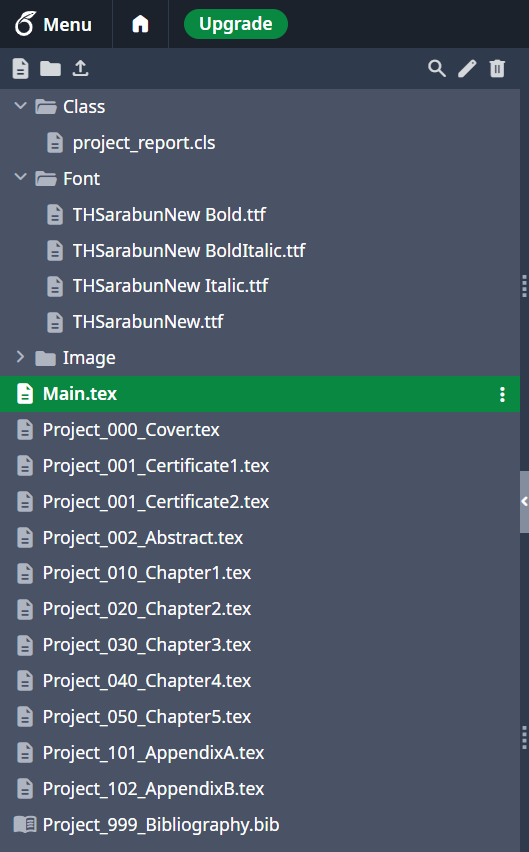
\includegraphics[width=0.6\textwidth]{Image/Structure_files.png}
}
\caption{\fontSixTeen{โครงสร้างไฟล์ทั้งหมด}}
\label{fig4:StructureFile}
\end{figure}

\hspace*{1.5em}
การจัดโครงสร้างไฟล์ในลักษณะนี้ไม่เพียงแต่ช่วยให้โปรเจกต์เป็นระเบียบ แต่ยังช่วยลดความซับซ้อนในการจัดการไฟล์จำนวนมาก ทำให้การทำงานเป็นทีมง่ายขึ้น และสามารถนำไปใช้งานต่อหรือแก้ไขในอนาคตได้อย่างสะดวกและมีประสิทธิภาพ